\chapter{Literature Survey}


This section will go over the general background knowledge I have acquired up until now to be able to produce educational content. It starts with a summary of the historical context behind quantum computing, before diving into quantum computing core concepts, phenomena, and algorithms.  

\section{ History and Context }

Quantum computing as a concept came about much longer ago than one would think. It began with Richard Feynman’s 1982 proposal that a machine based on quantum principles could simulate and mimic quantum systems (often specifically quantum mechanics) more effectively than classical systems\cite{Refrence2}. That was mainly for the purpose of helping us better understand the laws of physics and chemistry. Not long after, David Deutsch, often regarded as the father of quantum computing, introduced the 1985 concept of a universal quantum computer, laying foundational theory for the field. Peter Shor's 1994 algorithm demonstrated quantum computing's disruptive potential in cryptography, and then Lov Grover’s 1996 search algorithm provided a quadratic speedup compared to classic algorithmic equivalents.\newline

Up until 1998, quantum computing was theoretical and a physical quantum computer did not exist. All aforementioned researchers and scientists based and verified their research and algorithms on theoretical models of quantum computers, mathematical models and proofs and classical simulations.  This can be seen in Shor's paper "Algorithms for Quantum Computation: Discrete Logarithms and Factoring," where he proves his algorithm purely through mathematical proof \cite{Reference3}. \newline

In 1998, IBM and Stanford developed the first two-qubit quantum computer, proving real-world feasibility, and  providing the first experimental validation that those theoretical algorithms could work on real hardware. Different quantum designs, such as quantum annealers and quantum gate-based computers, were introduced in the 2000s and were each suitable for specific types of computation. In 2011, D-Wave launched the first commercial quantum computer, the D-Wave One, which was a quantum annealer designed specifically for optimisation, marking the beginning of quantum computing's commercialization. \newline 

Google claimed quantum supremacy in 2019 with its Sycamore processor, solving a problem in seconds that would take classical computers millennia. Despite rapid expansion in the 2020s, challenges such as scalability, qubit coherence, and noise reduction continue to hinder progress. Finally, current and future focus seems to be on quantum-classical hybrid models, promising advancements in cryptography, optimization, and secure communications.

\section{Quantum Computing Fundementals}

\subsection{The Qubit}

Starting with the most basic unit of a quantum computing system, we have the \textbf{qubit}. This is the equivalent of the classical bit, but it has the unique property of \textbf{superposition}, allowing it to exist in a combination of both 0 and 1 states simultaneously. This property is the foundational concept that makes quantum computing so powerful and fundamentally different from classical computing. \newline

The qubit is visually and mathematically represented using a \textbf{bloch sphere} pictured below in Figure 1. 

\begin{figure}[ht]
\centering
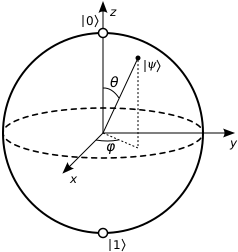
\includegraphics[width=5cm]{images/Bloch_sphere.svg.png}
\caption{A bloch sphere}
\end{figure}

Do not fear the bloch sphere. It is actually quite simple. To reiterate, a qubit can exist in an infinite array of combinations of the $|0\rangle$ and $|1\rangle$ states simultaneously\cite{refrence4}. Mathematically, a qubit state, represented in bra-ket notation as $|\psi\rangle$, can be written as a linear combination of the basis states $|0\rangle$ and $|1\rangle$ as follows:
 
 \vspace{0.01cm} 
\large
\begin{equation}
  |\psi\rangle = \alpha |0\rangle + \beta |1\rangle
\end{equation}
\normalsize 
\vspace{0.01cm} 

whereas $\alpha$ and $\beta$ are complex number representing the probability amplitude of the states $|0\rangle$ and $|1\rangle$, respectively. As such, the probability of measuring the qubit in state 0 will be $|\alpha|^2$, and the probability of measuring it in state 1 will be $|\beta|^2$. These amplitudes need to satisfy the normalization condition $\alpha^2 + \beta^2 = 1$, ensuring that the total probability is conserved.  Because $\alpha$ and $\beta$ can take on infinitely many values within this constraint, the qubit can exist in an infinite range of states between 0 and 1, covering every point on the Bloch sphere’s surface. Recall that a sphere has infinte points.\\ 

Using spherical coordinates with angles $\theta$ and $\phi$, each qubit state can be represented as a point on the surface of the Bloch sphere. Here, $\theta$ indicates the "latitude," showing the degree of superposition between the 0 and 1 states, while $\phi$ represents the "longitude," showing the relative phase between these states. This mapping helps us easily visualize quantum states, rotations, and transformations, making it simpler to study the effects of quantum gates and the behavior of qubits. 


\subsection{Common Qubit States}

Now that we understand what a qubit and a bloch sphere is, we can introduce some common qubit states, pictured below in Figure 2.2:

\begin{figure}[ht]
\centering
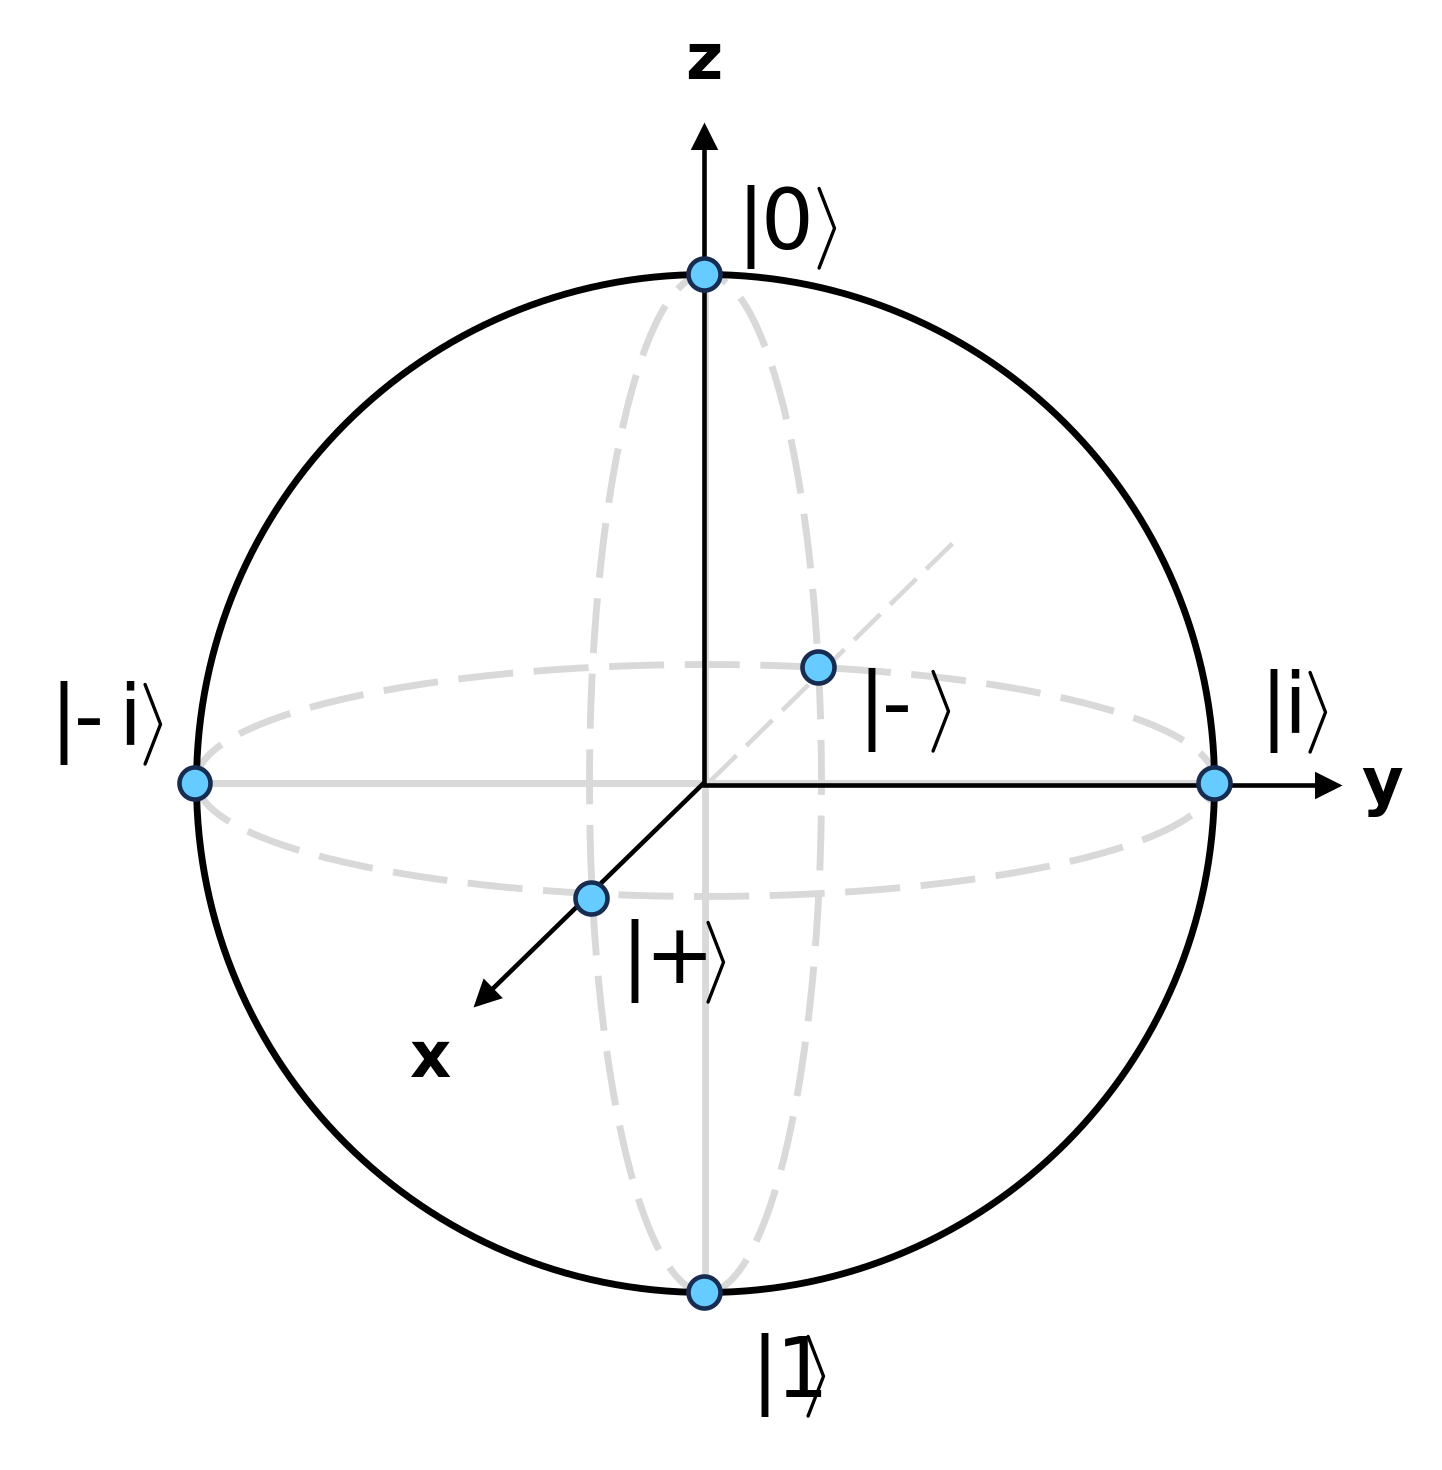
\includegraphics[width=7cm]{images/commonstatesbloch.png}
\caption{A bloch sphere with common qubit states}
\end{figure}

There are some commmon states represented as points along the X, Y and Z axes, each corresponding to a unique combination of $|0\rangle$ and $|1\rangle$ state probabilities. Note that a quantum state can also be represented as a complex vector. These points are spread out as follows: 

% \begin{itemize}
%     \item \textbf{Poles:} The north pole represents the state pure $|0\rangle$ with vector $\begin{pmatrix} 1 \\ 0 \end{pmatrix}$ such that it has a probability of 1. Similarly, the south pole represents the pure state \( |1\rangle \) with vector \( \begin{pmatrix} 0 \\ 1 \end{pmatrix} \), meaning it has a probability of 1 of being measured as 1. These two poles are the classical states of a qubit, with no superposition involved. Any state along the axis between these poles represents a superposition of \( |0\rangle \) and \( |1\rangle \) with varying probabilities.
%     \item \textbf{Equatorial Points:} Points on the equator of the Bloch sphere represent equal superpositions of \( |0\rangle \) and \( |1\rangle \) with different phases. For example:
%     \begin{itemize}
%         \item The point along the positive x-axis represents the state \( |+\rangle = \frac{1}{\sqrt{2}}(|0\rangle + |1\rangle) \).
%         \item The point along the negative x-axis represents the state \( |-\rangle = \frac{1}{\sqrt{2}}(|0\rangle - |1\rangle) \).
%     \end{itemize}
% \end{itemize} 



\begin{itemize}[noitemsep]
    \item \textbf{Poles:} The poles represent the pure states with definite outcomes. These two poles are the classical states of a qubit, with no superposition involved.
    \begin{itemize}
        \item \textbf{North:} represents the state \( |0\rangle \) with vector \( \begin{pmatrix} 1 \\ 0 \end{pmatrix} \), where P(0) = 1.
        \item \textbf{South:} represents the state \( |1\rangle \) with vector \( \begin{pmatrix} 0 \\ 1 \end{pmatrix} \), where P(1) = 1.
    \end{itemize}

    \item \textbf{Equatorial Points:} Points on the equator represent equal superpositions of \( |0\rangle \) and \( |1\rangle \) (i.e. P(0) = P(1) = 0.5) with different \textbf{phases}. 
    \begin{itemize}[label=$\circ$]
        \item \textbf{+ve x-axis:} represents \( |+\rangle = \frac{1}{\sqrt{2}}(|0\rangle + |1\rangle) \), with vector \( \begin{pmatrix} \frac{1}{\sqrt{2}} \\ \frac{1}{\sqrt{2}} \end{pmatrix} \).
        
        \item \textbf{-ve x-axis:} represents \( |-\rangle = \frac{1}{\sqrt{2}}(|0\rangle - |1\rangle) \), with vector \( \begin{pmatrix} \frac{1}{\sqrt{2}} \\ -\frac{1}{\sqrt{2}} \end{pmatrix} \). 
        
        \item \textbf{+ve y-axis:} represents \( |+i\rangle = \frac{1}{\sqrt{2}}(|0\rangle + i|1\rangle) \), with vector \( \begin{pmatrix} \frac{1}{\sqrt{2}} \\ \frac{i}{\sqrt{2}} \end{pmatrix} \). 
        
        \item \textbf{-ve y-axis:} represents \( |-i\rangle = \frac{1}{\sqrt{2}}(|0\rangle - i|1\rangle) \), with vector \( \begin{pmatrix} \frac{1}{\sqrt{2}} \\ -\frac{i}{\sqrt{2}} \end{pmatrix} \). 
    \end{itemize}
\end{itemize}

The difference between these equatorial points is their phase. Phase refers to the "angle" of each state relative to others, which affects how the states combine or interfere with one another. Although all these points have a 50\% chance of measuring either 0 or 1, their phases determine whether they align or cancel each other out when combined with other qubits. For example:
\begin{itemize}
    \item The state on the positive x-axis \( |+\rangle \) has no phase difference between 0 and 1, meaning both parts are "in sync."
    \item The state on the negative x-axis \( |-\rangle \) has a phase shift of 180 degrees, so the 0 and 1 parts are out of sync.
    \item The states on the y-axis \( |+i\rangle \) and \( |-i\rangle \) have phase shifts of 90 degrees and -90 degrees, creating different "rotations" of the state.
\end{itemize} 
\vspace{0.1cm}

\begin{tcolorbox}[colback=gray!5!white, colframe=gray!75!black, title=Note on \(i\)]
The imaginary unit \( i \) is defined as \( i = \sqrt{-1} \), meaning \( i^2 = -1 \). Complex numbers  of the form \( a + bi \), where \( a \) is the real part, and \( b \) is the imaginary part. In quantum computing, they are used to describe quantum states, with the real and imaginary parts encoding both the amplitude (probability) and the phase (relative orientation) of a state. The phase, often involving \( i \), determines how quantum states combine and interfere during computations.
\end{tcolorbox}


\subsection{Measuring the Qubit}

In the previous section, we explored the Bloch sphere, which provides a visual representation of a qubit's state as a point in a three-dimensional space. However, when we measure a qubit, this state collapses to one of the two basis states: \( |0\rangle \) or \( |1\rangle \). The probabilities of measuring these states depend on the position of the qubit on the Bloch sphere.For example,  consider a qubit in the superposition state:
\vspace{0.1em}
\[
|\psi\rangle = \frac{2 + 3i}{\sqrt{13}} |0\rangle + \frac{1 - 2i}{\sqrt{13}} |1\rangle
\]
\vspace{0.1em}On the Bloch sphere, this qubit lies closer to the \( |1\rangle \) state than to the \( |0\rangle \) state, indicating that it is more likely to collapse to \( |1\rangle \) upon measurement. We cannot be certain of the qubit's state until we measure it. Once measured, however, the qubit collapses to a definite state, and its value is no longer probabilistic—it becomes a fixed, observable outcome.


\subsection{Quantum Gates}

Just like classical computing, quantum also has gates that affect the state of its foundational unit, the Qubit. Figure 2.3 and Table 2.1 below illustrate the representations used to denote quantum gates and their respective functions 


\begin{figure}[ht]
\centering
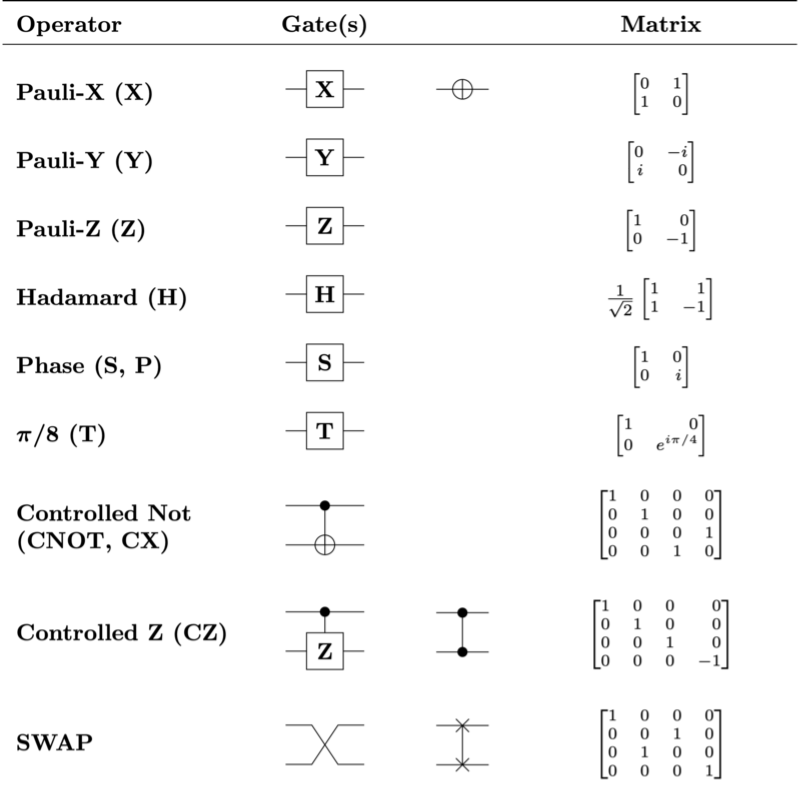
\includegraphics[width=10cm]{images/Quantum_Logic_Gates.png}
\caption{Quantum gates, Source: Rxrtreme, CC BY-SA 4.0, via Wikimedia Commons.}
\end{figure}


\begin{table}[h]
    \centering
    \begin{tabular}{|c|p{9cm}|p{3cm}|}
        \hline
        \textbf{Gate} & \textbf{Description} & \textbf{Example Effect} \\
        \hline
        Pauli-X (X) & Bit-flip gate, like a classical NOT operation.  & \parbox{7cm}{\( X|0\rangle = |1\rangle \\ X|1\rangle = |0\rangle \)} \\
        \hline
        Pauli-Z (Z) & Phase-flip gate; leaves \( |0\rangle \) unchanged and flips the phase of \( |1\rangle \) to \( -|1\rangle \). & \parbox{7cm}{\( Z|0\rangle = |0\rangle \\ Z|1\rangle = -|1\rangle \)} \\
        \hline
        Pauli-Y (Y) & Combines a bit-flip with a phase-flip. It flips the state and adds a \( \pi \) phase. & \parbox{7cm}{\( Y|0\rangle = i|1\rangle \\ Y|1\rangle = -i|0\rangle \)} \\
        \hline
        Hadamard (H) & Creates a superposition. Maps \( |0\rangle \) to an equal superposition of \( |0\rangle \) and \( |1\rangle \). & \parbox{7cm}{\( H|0\rangle = \frac{|0\rangle + |1\rangle}{\sqrt{2}} \\ H|1\rangle = \frac{|0\rangle - |1\rangle}{\sqrt{2}} \)} \\
        \hline
        Phase (S) & Adds a phase of \( \frac{\pi}{2} \) to the \( |1\rangle \) state, leaving \( |0\rangle \) unchanged. & \parbox{7cm}{\( S|0\rangle = |0\rangle \\ S|1\rangle = i|1\rangle \)} \\
        \hline
        \( \pi/8 \) (T) & Adds a phase of \( \frac{\pi}{4} \) to the \( |1\rangle \) state. Often used in phase-shift operations. & \parbox{7cm}{\( T|0\rangle = |0\rangle \\ T|1\rangle = e^{i\pi/4}|1\rangle \)} \\
        \hline
        CNOT (CX) & Controlled-NOT gate: flips the target qubit if the control qubit is \( |1\rangle \). Commonly used for entangling qubits. & \parbox{7cm}{\( \text{CNOT}|10\rangle = |11\rangle \\ \text{CNOT}|00\rangle = |00\rangle \)} \\
        \hline
        Controlled-Z (CZ) & Controlled phase-flip: applies a Z gate to the target qubit only if the control qubit is \( |1\rangle \). & \parbox{7cm}{\( \text{CZ}|11\rangle = -|11\rangle \\ \text{CZ}|10\rangle = |10\rangle \)} \\
        \hline
        SWAP & Swaps the states of two qubits. Useful for reordering qubits in quantum circuits. & \parbox{7cm}{\( \text{SWAP}|01\rangle = |10\rangle \\ \text{SWAP}|10\rangle = |01\rangle \)} \\
        \hline
    \end{tabular}
    \caption{Quantum gates, their descriptions, and example effects}
\end{table}


\subsection{Entanglement}

Quantum entanglement is a unique and fundamental phenomenon in quantum mechanics, where two or more qubits become interconnected in such a way that the state of one qubit is directly related to the state of the other(s), regardless of the physical distance between them. This means that measuring one qubit instantly determines the state of its entangled partner(s), even if they are separated by vast distances.\\

Figure 2.4 illustrates a common circuit used to create a basic quantum entanglement between two qubits, \( q_0 \) and \( q_1 \). The circuit consists of two operations: a \textbf{Hadamard gate} on \( q_0 \) and a \textbf{Controlled-NOT (CNOT) gate} between \( q_0 \) and \( q_1 \). Note that here we introduce a two qubit system for the first time. \newpage

\begin{figure}[ht]
\centering
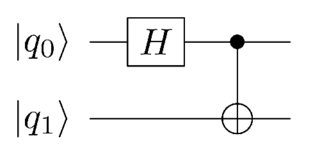
\includegraphics[width=7cm]{images/cnot.jpg}
\caption{Entaglement using CNOT (Bell state  circuit).}
\end{figure}

\begin{itemize}
    \item \textbf{Hadamard Gate (H):} The Hadamard gate is applied to qubit \( q_0 \), placing it in a superposition state. If \( q_0 \) starts in the \( |0\rangle \) state, applying the Hadamard gate will create a superposition state \( \frac{1}{\sqrt{2}}(|0\rangle + |1\rangle) \), meaning \( q_0 \) now has equal probabilities of being measured as \( |0\rangle \) or \( |1\rangle \).
    
    \item \textbf{Controlled-NOT (CNOT) Gate:} The CNOT gate is then applied with \( q_0 \) as the control qubit and \( q_1 \) as the target qubit. This gate flips the state of \( q_1 \) if \( q_0 \) is in the \( |1\rangle \) state, entangling the two qubits. As a result, the combined state of \( q_0 \) and \( q_1 \) becomes \( \frac{1}{\sqrt{2}}(|00\rangle + |11\rangle) \), an entangled state known as a Bell state. 
\end{itemize}

In this entangled state, measuring \( q_0 \) will instantly determine the state of \( q_1 \), and vice versa. If \( q_0 \) is measured as \( |0\rangle \), \( q_1 \) will also be \( |0\rangle \); if \( q_0 \) is measured as \( |1\rangle \), \( q_1 \) will also be \( |1\rangle \). This entanglement allows the two qubits to share information in a way that cannot be achieved in classical systems.


\subsection{Quantum Circuits}
\subsection{Interesting Quantum Phenomenon}

\subsection{Quantum Noise and Error Correction }

\subsection{Classical Quantum Simulation and Qiskit}


\subsection{Shor's Factorisation Algortihm }

\subsection{Grover's Search Algorithm }

\subsection{Quantum Complexity: P, NP and BQP}

\newpage

\section{Existing Tools}

\subsection{General tools}
\subsection{Lea Button's simulator}

\section{Technology survey}

Lorem ipsum dolor sit amet, consectetuer adipiscing elit. Aenean commodo ligula eget dolor. Aenean massa. Cum sociis natoque penatibus et magnis dis parturient montes, nascetur ridiculus mus. Donec quam felis, ultricies nec, pellentesque eu, pretium quis, sem. Nulla consequat massa quis enim. Donec pede justo, fringilla vel, aliquet nec, vulputate eget, arcu. In enim justo, rhoncus ut, imperdiet a, venenatis vitae, justo. Nullam dictum felis eu pede mollis pretium. Integer tincidunt. Cras dapibus. Vivamus elementum semper nisi. Aenean vulputate eleifend tellus. Aenean leo ligula, porttitor eu, consequat vitae, eleifend ac, enim. Aliquam lorem ante, dapibus in, viverra quis, feugiat a, tellus. Phasellus viverra nulla ut metus varius laoreet. Quisque rutrum. Aenean imperdiet. Etiam ultricies nisi vel augue. Curabitur ullamcorper ultricies nisi. Nam eget dui. Etiam rhoncus. Maecenas tempus, tellus eget condimentum rhoncus, sem quam semper libero, sit amet adipiscing sem neque sed ipsum. Nam quam nunc, blandit vel, luctus pulvinar, hendrerit id, lorem. Maecenas nec odio et ante tincidunt tempus. Donec vitae sapien ut libero venenatis faucibus. Nullam quis ante. Etiam sit amet orci eget eros faucibus tincidunt. Duis leo. Sed fringilla mauris sit amet nibh. Donec sodales sagittis magna. Sed consequat, leo eget bibendum sodales, augue velit cursus nunc.
